\documentclass{article}

\usepackage{hyperref}
\hypersetup{
	colorlinks=true,
	linkcolor=blue,
	filecolor=magenta,      
	urlcolor=cyan
}
\usepackage[american]{circuitikz}
\ctikzset{tripoles/mos style/arrows}
\ctikzset{transistors/arrow pos=end}
\ctikzset{label/align = straight}
\usepackage{siunitx}
\usepackage{amsmath}

\begin{document}
	This document describes how a BJT works in active mode at the electron movement level.
	The understanding is gained by reading \textit{Sedra \& Smith Microelectronics Circuits, Chapter 6.1.1 and 6.1.2}. We will be using a NPN transistor as example.
	\section{Biasing}
		So there is the collector-base junction(CBJ) and the emitter-base junction(EBJ). In active mode, EBJ has to be forward biased and CBJ has to be reversed biased. See the picture below
		\begin{center}
			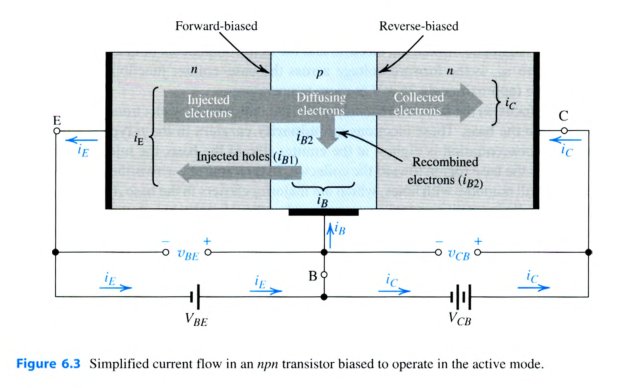
\includegraphics[width=\textwidth]{img/npn_active_mode.png}
		\end{center}
	\section{PN junction}
		This picture will help visualize things
		\begin{center}
			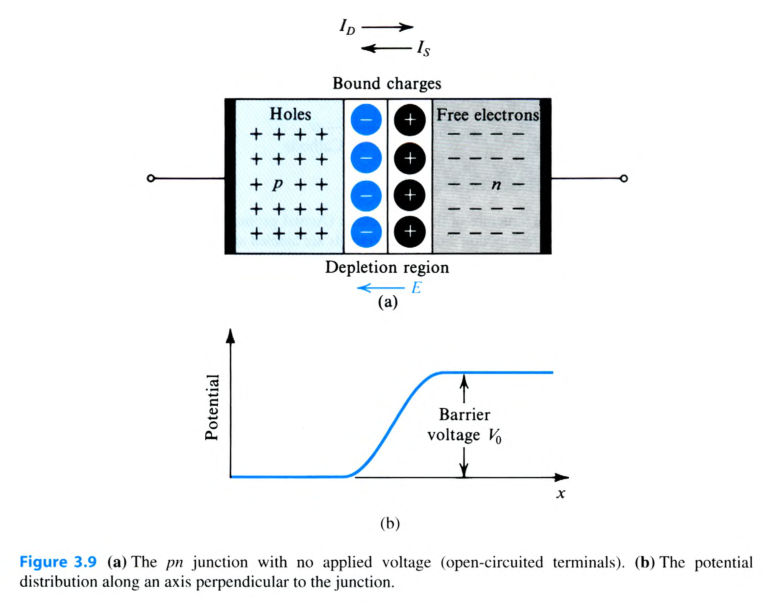
\includegraphics[width=\textwidth]{img/pn_junction_equilibrium.png}
		\end{center}
		Remember that Lorentz Force Law is given by
		\begin{align*}
			\vec{F}&=q\vec{E}+q\vec{v}\times\vec{B}\\
			q&=charge\\
			\vec{E}&=eletric field\\
			\vec{v}&=velocity\\
			\vec{B}&=magnetic field
		\end{align*}
		We'll just look at the electric field component, \[\vec{F}=q\vec{E}\]$q$ is positive for positive charge and negative for negative charge. Following the picture of the pn junction above we set left side to be positive, right side to be negative.
	\section{How Electrons Flow and Creates Base/Collector Current}
		Now what we have established DC bias, when a small signal increasing input (voltage or current honestly you can say either) at the base terminal, electrons are injected at the emitter terminal. Because EBJ is forward biased, electrons at n side(emitter) goes across to the p side(base). Here some electrons are combined with the holes that were already in the base. Every time a hole combines with a electron, new holes needs to be supplied from outside of the base terminal(electrons coming out of the base terminal), thus a base current is present.\\
		Now majority of those electrons in base region will get swept across to collector region, this is because CBJ is reversed biased(looks like the picture of the PN junction), the electric field is pointing from collector to base. Electrons are negative charges, they experience force in the opposite direction of the electric field, thus they go over to collector. The amount of electrons going over to collector is proportional to the amount of electrons that makes it across EBJ from emitter. Which is why the collector current is given by
		\begin{align}
			\label{eq:1}
			i_c=I_{s}e^{v_{BE}/V_{T}}
		\end{align}
		See that equation \ref{eq:1} depends on $v_{BE}$ and not $v_{CB}$. As long as the collector voltage is higher than the voltage at the base, those electrons will get swept across, doesn't matter the magnitude.
\end{document}